%Version 2.1 April 2023
% See section 11 of the User Manual for version history
%
%%%%%%%%%%%%%%%%%%%%%%%%%%%%%%%%%%%%%%%%%%%%%%%%%%%%%%%%%%%%%%%%%%%%%%
%%                                                                 %%
%% Please do not use \input{...} to include other tex files.       %%
%% Submit your LaTeX manuscript as one .tex document.              %%
%%                                                                 %%
%% All additional figures and files should be attached             %%
%% separately and not embedded in the \TeX\ document itself.       %%
%%                                                                 %%
%%%%%%%%%%%%%%%%%%%%%%%%%%%%%%%%%%%%%%%%%%%%%%%%%%%%%%%%%%%%%%%%%%%%%

\documentclass[sn-basic,Numbered,pdflatex]{sn-jnl}

%%%% Standard Packages
%%<additional latex packages if required can be included here>

\usepackage{graphicx}%
\usepackage{multirow}%
\usepackage{amsmath,amssymb,amsfonts}%
\usepackage{amsthm}%
\usepackage{mathrsfs}%
\usepackage[title]{appendix}%
\usepackage{xcolor}%
\usepackage{textcomp}%
\usepackage{manyfoot}%
\usepackage{booktabs}%
\usepackage{algorithm}%
\usepackage{algorithmicx}%
\usepackage{algpseudocode}%
\usepackage{listings}%
%%%%

%%%%%=============================================================================%%%%
%%%%  Remarks: This template is provided to aid authors with the preparation
%%%%  of original research articles intended for submission to journals published
%%%%  by Springer Nature. The guidance has been prepared in partnership with
%%%%  production teams to conform to Springer Nature technical requirements.
%%%%  Editorial and presentation requirements differ among journal portfolios and
%%%%  research disciplines. You may find sections in this template are irrelevant
%%%%  to your work and are empowered to omit any such section if allowed by the
%%%%  journal you intend to submit to. The submission guidelines and policies
%%%%  of the journal take precedence. A detailed User Manual is available in the
%%%%  template package for technical guidance.
%%%%%=============================================================================%%%%

\usepackage{pdflscape}
\usepackage{booktabs}
\usepackage{caption}
\usepackage{longtable}
\usepackage{colortbl}
\usepackage{array}
\usepackage{anyfontsize}


\raggedbottom

\unnumbered



% tightlist command for lists without linebreak
\providecommand{\tightlist}{%
  \setlength{\itemsep}{0pt}\setlength{\parskip}{0pt}}

% From pandoc table feature
\usepackage{longtable,booktabs,array}
\usepackage{calc} % for calculating minipage widths
% Correct order of tables after \paragraph or \subparagraph
\usepackage{etoolbox}
\makeatletter
\patchcmd\longtable{\par}{\if@noskipsec\mbox{}\fi\par}{}{}
\makeatother
% Allow footnotes in longtable head/foot
\IfFileExists{footnotehyper.sty}{\usepackage{footnotehyper}}{\usepackage{footnote}}
\makesavenoteenv{longtable}




\begin{document}


\title[]{Substitution of red meat with legumes and risk of primary liver cancer in 126,744 UK Biobank participants a prospective cohort study}

%%=============================================================%%
%% Prefix	-> \pfx{Dr}
%% GivenName	-> \fnm{Joergen W.}
%% Particle	-> \spfx{van der} -> surname prefix
%% FamilyName	-> \sur{Ploeg}
%% Suffix	-> \sfx{IV}
%% NatureName	-> \tanm{Poet Laureate} -> Title after name
%% Degrees	-> \dgr{MSc, PhD}
%% \author*[1,2]{\pfx{Dr} \fnm{Joergen W.} \spfx{van der} \sur{Ploeg} \sfx{IV} \tanm{Poet Laureate}
%%                 \dgr{MSc, PhD}}\email{iauthor@gmail.com}
%%=============================================================%%

\author*[1]{\fnm{Niels} \sur{Bock} }\email{\href{mailto:nb@ph-au.dk}{\nolinkurl{nb@ph-au.dk}}}

\author[1]{\fnm{Fie} \sur{Langmann} }

\author[1]{\fnm{Christina} \spfx{C.} \sur{Dahm} }



  \affil*[1]{\orgdiv{Department of Public Health}, \orgname{Aarhus University}, \orgaddress{\city{Aarhus}, \country{Denmark}}}

\abstract{\textbf{Purpose}: Lifestyle-associated primary liver cancer is on the rise worldwide. Preventative strategies are warranted. We aimed to estimate the effect of substituting unprocessed red meat, processed red meat and total red meat with legumes on primary liver cancer in a free-living population.

\textbf{Methods}: We analyzed data from 126,744 UK Biobank participants who completed \(\geq\) 2 24-hour diet recall questionnaires. Cox proportional hazards regression models were used to estimate substitution of 15g/day of legumes with 15/day of total red meat, unprocessed red meat and processed red meat on liver cancer risk, using the leave-one-out food substitution model. Baseline characteristics were collected from the initial assessment visit. Information on liver cancer diagnoses was collected via external linkage to inpatient hospital episodes or central cancer registries.

\textbf{Results}: During a median follow-up time of 11.3 years, 173 participants developed liver cancer. In the fully adjusted models, no effect of substituting 15/day of legumes with total red meat (HR: 0.98 (95\% CI 0.93-1.04)), unprocessed red meat (HR: 0.97 (95\% CI 0.91-1.03)) or processed red meat (HR: 1.02 (95\% CI 0.93-1.13)) was observed. The results were robust to sensitivity analyses.

\textbf{Conclusion}: Overall, no association between substituting red meat with legumes and liver cancer was observed. Further research with longer follow-up time is warranted.}

\keywords{Food Substitutions, Liver cancer, Red meat, Legumes}



\maketitle

\hypertarget{sec1}{%
\section{Background}\label{sec1}}

The main aim of this study was to estimate the effect of substituting
unprocessed red meat, processed red meat and total red meat with legumes
on primary liver cancer in a free-living population.

\hypertarget{sec2}{%
\section{Research Design and Methods}\label{sec2}}

\hypertarget{subsec1}{%
\subsection{Study population}\label{subsec1}}

The UK Biobank, a population-based prospective cohort, was initiated in
2006. \citep{sudlow2015} During 2006-2010, more than 500,000 participants,
aged 40-69, were recruited and visited designated assessment centres
across the UK Participants provided information about age, sex,
sociodemographic factors (education, Townsend deprivation index, living
alone) and lifestyle factors (smoking, alcohol consumption, physical
activity) via touch screen questionnaires and computer-assisted
interviews. Anthropometric data (waist circumference) were collected via
physical measurements \citep{RN113}.

\hypertarget{subsec2}{%
\subsection{Dietary assessment}\label{subsec2}}

A web-based 24-hour dietary recall was administered at the end of the
initial assessment visit for the last 70,000 recruited participants
\citep{RN115}. From February 2011 to April 2012, 320,000 participants who had
provided an e-mail address were invited on four separate occasions to
complete the 24-hour dietary recall, the Oxford WebQ, of which 210,947
participants completed at least one. The Oxford WebQ covered 206 food
items and 32 beverage items commonly consumed in the UK. Intakes were
reported in standard units of measurements, e.g., servings, cups,
slices, etc. with intake categories ranging from 0 to 3+ units
\citep{piernas2021}. The Oxford WebQ has been validated against
interviewer-based 24-hour dietary recalls and biomarkers \citep{Liu2011, Greenwood2019}.

Researchers defined79 food groups and 14 beverage groups from the Oxford
WebQ using the UK National Diet and Nutrition Survey categories
\citep{piernas2021}. These food and beverage groups were used when defining
the food groups used in the substitution analyses (Supplementary Table
1). Legumes were defined as dietary pulses, baked beans, tofu-based
products, peas, hummus, soy drinks, and soy-based desserts and yogurt.
Red meat intake was defined as intake of beef, pork, lamb, or other
meat, including offal. Processed red meat intake was defined as
sausages, bacon (with and without fat), ham, or liver pate. Other food
groups included were animal-based foods, unhealthy plant-based foods,
healthy plant-based foods, and alcoholic beverages (Supplementary Table
1). Animal-based and healthy and unhealthy plant-based food foods were
grouped based on plant-based diet indices from previous studies
\citep{Thompson2023, Heianza2021, Satija2017, Satija2016}. An overview of
included foods in each food group is displayed in Supplementary Table 1.

Due to the incapability of a single 24-hour dietary recall to properly
assess habitual dietary intake and variation in diet over time
\citep{thompson2013, gurinovic2017}, only participants who completed two or
more Oxford WebQs were eligible for inclusion in this study.

\hypertarget{subsec3}{%
\subsection{Liver cancer assessment}\label{subsec3}}

Liver cancer was defined according to ICD-10 diagnosis codes C22.0 for
Hepatocellular carcinoma (HCC) or C22.1 for Intrahepatic
cholangiocarcinoma (ICC) and ICD-9 diagnosis codes 1550 Malignant
neoplasm of liver, primary or 1551 Malignant neoplasm of intrahepatic
bile ducts. Incident and prevalent cases of liver cancer and
corresponding diagnosis dates were obtained via external linkage to
central cancer registries or hospital inpatient episodes \citep{RN112, RN114}.

\hypertarget{subsec4}{%
\subsection{Assessment of confounders}\label{subsec4}}

Confounders were defined \emph{a priori} from a literature review of the
background literature and illustrated using directed acyclic graphs
(Supplementary Figure 1). The following confounding variables were
selected: age at baseline (years, continuous), sex (male, female),
educational level (high: College or University degree, intermediate: A
levels/AS levels, O levels/GCSEs, or equivalent, low: none of the
previous mentioned), Townsend Deprivation Index (continuous), Living
alone (yes, no), waist circumference (cm, continuous), physical activity
(above/below the 2017 UK Physical activity guidelines of 150 minutes of
moderate activity per week or 75 minutes of vigorous activity, or
unknown), smoking (pack years as a proportion of lifespan exposed to
smoking, continous), and alcohol intake (g/day, continuous). All
confounders except age were selected from the initial assessment visit
before the start of follow-up.

\hypertarget{subsec5}{%
\subsection{The substitution model}\label{subsec5}}

The substitution analyses were conducted by replacing an equal mass of
meat with legumes. The size of the substitution was set to 15 g of
legumes for 15 g of meat to keep the substitution size below the mean
intake of any of the substituted food groups in the cohort. The
substitutions were modeled using the leave-one-out-approach in which
variables for every food group along with a variable for total food
intake are included, except the food group that are to be substituted
\citep{Ibsen2021}. To estimate substitution of 15 g of all red meats (red and
processed) with 15 g of legumes, the following model was defined:

\begin{align}
\log(h(t;x)) &= \log(h_0(t)) + \beta_1 \text{Legumes (15g)} + \beta_2 \text{Total food intake (g)} \nonumber \\
&\quad + \beta_3 \text{Other food groups (g)} + \beta_4 \text{Covariates}
\end{align}

\noindent When substituting only red meat with legumes, processed red
meat was added to the model:

\begin{align}
\log(h(t;x)) &= \log(h_0(t)) + \beta_1 \text{Legumes (15g)} + \beta_2 \text{Processed red meat (15g)} \nonumber \\
&\quad + \beta_3 \text{Total food intake (g)} + \beta_4 \text{Other food groups (g)} \nonumber \\
&\quad + \beta_5 \text{Covariates}
\end{align}

\noindent When substituting only processed red meat with legumes, red
meat was added to the model:

\begin{align}
\log(h(t;x)) &= \log(h_0(t)) + \beta_1 \text{Legumes (15g)} + \beta_2 \text{Red meat (15g)} \nonumber \\
&\quad + \beta_3 \text{Total food intake (g)} + \beta_4 \text{Other food groups (g)} \nonumber \\
&\quad + \beta_5 \text{Covariates}
\end{align}

\noindent The performance of the leave-one-out model when modeling equal
mass substitutions has been validates against simulated data
\citep{Tomova2022}.

\hypertarget{subsec6}{%
\subsection{Statistical analysis}\label{subsec6}}

Multivariable-adjusted Cox proportional hazards regression models were
used to estimate hazard ratios (HR) with corresponding 95\% confidence
intervals (CI) with age as the underlying timescale. Participants were
followed from the date of their last completed Oxford WebQ until the
occurrence of the event of interest or due to right censoring, whichever
came first. Participants were right censored in the event of death, loss
to follow-up, or administrative end of follow-up (October 31, 2022). Two
levels of adjustments were added to the substitution model. Model 1 was
minimally adjusted for age, total weight of food intake, and all other
food groups to fit the substitution model. Model 2 was further adjusted
for sex, educational level, Townsend Deprivation Index, living alone,
physical activity, smoking, alcohol intake, and waist circumference.

In secondary analyses, each cancer type was analysed separately to
evaluate if the pooling of HCC and ICC as one outcome in the main
analysis was justified. Furthermore, to estimate the effect of legume
intake regardsless of other dietary components, legume consumers
(divided into quartiles) were compared to non-consumers.

To evaluate the robustness of the main analyses, sensitivity analyses
were performed on subsamples of participants by excluding those with
high alcohol intake (exclusion of upper decile of daily alcohol intake
for each sex), implausible energy intake (exclusion of upper and lower
deciel of each sex), any liver disease before baseline, any type of
cancer before baseline, and fewer than 3 completed Oxford WebQs. As
neither the central cancer registries nor the hospital inpatient
registries were complete, liver cancer diagnoses retrieved from death
registries, which where more up-to-date, were included in a sensitivity
analysis to test for outcome misclassification bias. Lastly, one of our
causal assumptions was that anthropometry confounded the causal
relationship between replacing red meat with legumes and liver cancer;
however, strong arguments exist giving support to anthropometry being a
mediator between diet and health outcomes. Thus, to test for erroneously
conditioning on a potential mediator, waist circumference was removed in
a sensitivity analysis. Sensitivity analyses were modeled like the fully
adjusted models in the main analyses.

All analyses were conducted in R (version 4.1.1) with a significance
level of 5 \%.

\hypertarget{sec3}{%
\section{Results}\label{sec3}}

After excluding participants with liver cancer before baseline,
participants lost to follow-up before baseline, and participants with
errors in the diet data, 126,744 participants remained who had completed
two or more diet questionnaires (Figure \ref{fig:fig1}).

\begin{figure}[b]
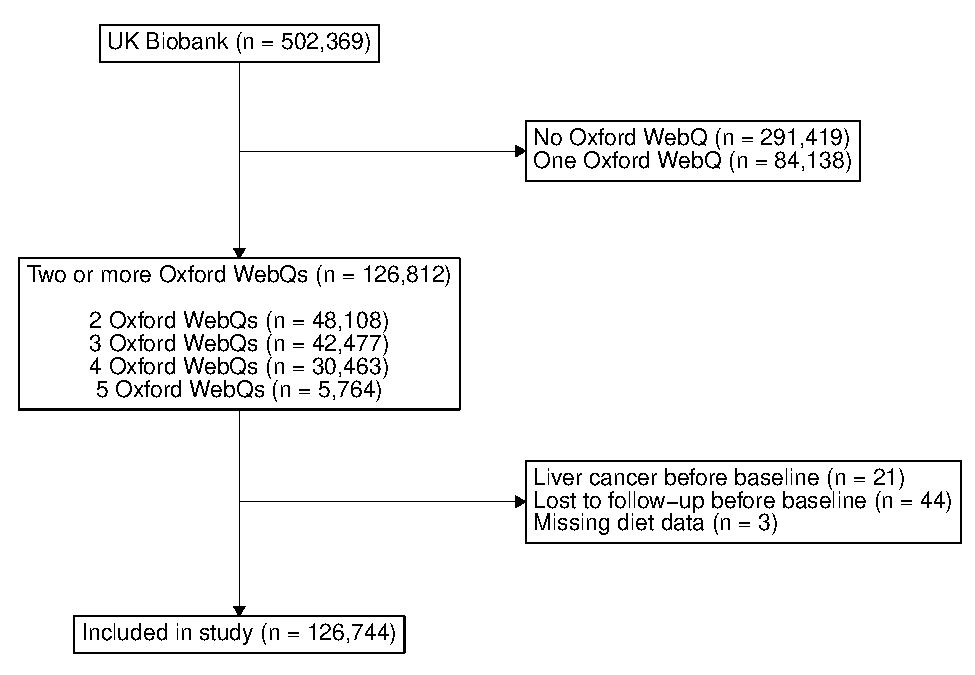
\includegraphics[width=1\linewidth,]{Springer-test_files/figure-latex/fig1-1} \caption{Flowchart of included participants. Missing diet data were merged with loss to follow-up before baseline due to n being less than 5. It should be noted that not all UK Biobank participants were invited to complete an Oxfords WebQ. Only the last 70,000 participants to visit an assessment center were asked to complete an Oxford WebQ at the end of their visit. Further Oxfords WebQs were sent to ~320,000 participants who provied an e-mail adress.}\label{fig:fig1}
\end{figure}

During a median follow-up time of 11.3 years, 173 participants developed
liver cancer. Participants who developed liver cancer were older at
baseline, had a higher waist circumference, were less physically active,
fewer had never smoked, and more were male, compared to all included
participants (Table 1).

Mean daily energy intake and food intake and daily intake of all
specified food groups in grams are presented in table 2.

No association was found for substituting 15 g/day of legumes with 15
g/day of total red meat, unprocessed red meat, or processed red meat and
risk of primary liver cancer in model 1 (Table 3: total red meat:
HR: 0.98, 95\% CI: 0.93-1.04;
unprocessed red meat:
HR: 0.97, 95\% CI: 0.91-1.03;
processed red meat:
HR: 1.02, 95\% CI: 0.93-1.13).
The estimated associations changed minimally but remained
non-significant with further adjustments (Table 3: total red meat:
HR: 1.02, 95\% CI: 0.96-1.08;
unprocessed red meat:
HR: 1.00, 95\% CI: 0.94-1.07;
processed red meat:
HR: 1.09, 95\% CI: 0.98-1.20).

In secondary analyses, when analyzing the substitution association for
HCC and ICC separately, the risk of HCC was positively associated with
substituting total, unprocessed, or processed red meat with legumes
(Supplementary Table 2, total red meat:
HR: 1.06, 95\% CI: 0.97-1.16;
red meat:
HR: 1.05, 95\% CI: 0.96-1.15;
processed red meat:
HR: 1.09, 95\% CI: 0.95-1.26).
The association between substituting total or unprocessed red meat with
legumes and ICC indicated inverse associations (Supplementary Table 2:
total red meat:
HR: 0.97, 95\% CI: 0.90-1.05;
red meat:
HR: 0.95, 95\% CI: 0.87-1.03;
processed red meat:
HR: 1.07, 95\% CI: 0.93- 1.22).
The magnitude or direction of associations were not significantly
different across strata of liver cancer types.

In the adjusted non-substitution analysis, a mean intake of 6.3 grams of
legumes per day was associated with a reduced risk of liver cancer,
compared to no intake
(HR: 0.59, 95\% CI: 0.35-0.98);
however, no associations were observed with further increase in legume
intake (supplementary table 3).

In sensitivity analyses, excluding participants based on high alcohol
intake, implausible energy intake, any liver disease or cancer before
baseline, or fewer than 3 completed Oxford WebQs did not alter the
estimates in any statistically significant way. This also applied for
including death registries as a source of liver cancer events and
excluding waist circumference from the fully adjusted analysis
(Supplementary table 4).

\hypertarget{sec4}{%
\section{Discussion}\label{sec4}}

In this study of UK Biobank participants, we found no effect of
replacing 15g/day of red meat with legumes on risk of primary liver
cancer. The estimates did not change significantly in any of the
sensitivity analyses. When stratifying by liver cancer type, replacing
total red meat and unprocessed red meat with legumes showed an inverse
association with ICC, though the results were not statistically
significant.

Contrary to our hypothesis, replacing processed red meat with legumes
was associated with a non-significant increase in risk of primary liver
cancer, with a greater effect size compared to unprocessed red meat.
This pattern persisted across all sensitivity analyses. However, the
estimates for processed red meat were labeled with less confidence,
partly due to the low median intake. These findings align with recent
analyses from the UK Biobank, which indicated that unprocessed red meat
intake was associated with a non-significant increase in liver cancer
risk, with a greater effect size than processed meat (both white and red
meat) \citep{Knuppel2020}. This supports the notion that processed meat may
not be associated with liver cancer risk in this population.

Stratifying on cancer type revealed that replacing unprocessed red meat
with legumes to some extent was associated with a decreased risk of ICC,
contrary to HCC (Supplementary table 4). However, the robustness of
these results were not tested in further analyses as they were
associated with greater uncertainty.

The literature on food substitutions, particularly in relation to liver
cancer, is sparse. However, a recent meta-anlysis of observational
studies found a non-linear dose-response relationship between legume
intake and liver cancer risk, with a protective effect observed between
intakes of 8 g/day to 40 g/day \citep{liu2023a}. This somewhat contrasts with
our findings where any increase above 6.3 g/day of legumes was not
associated with a decreased risk of liver cancer, compared to no legume
intake. A recent meta-analysis of observational studies showed no
association between red or processed meat intake and HCC \citep{Di2023}.

This study had some limitations. First, None of the registries used to
determine a diagnosis of liver cancer were complete or up-to-date at the
time of analysis \citep{RN112}. Data from external providers, such as the NHS
England, NHS Central Register or National Records of Scotland, were
estimated to be mostly complete by the UK Biobank at various dates,
ranging from 31 December 2016 for cancer data from Wales to 31 October
2022 for hospital inpatient data from England \citep{RN114}. This could
introduce misclassification bias, as individuals with liver cancer may
not be identified as events. However, the estimates were robust in a
sensitivity analysis that included death registries as an additional
source of liver cancer diagnoses to accommodate missing outcome events.
Second, the relatively low number of events limited our ability to
adjust for confounding factors. Too many adjustment levels per event can
compromise the validity of the multivariable Cox regression model,
potentially causing biased estimates. To ensure statistical validity, we
aimed for at least 10 events per variable in the main analysis by
limiting the number of adjustment levels, using fewer and broader food
groups, and fewer levels for categorical covariates. This approach was
guided by our \emph{a priori} causal assumptions. Although this method helped
maintain statistical validity, it may have increased residual
confounding by diluting the importance of specific food groups.
Additionally, risk factors that we could not adjust for, such as
aflatoxin B1, a known liver carcinogen, may have contributed to residual
confounding.

Strengths of this study are the prospective longitudinal design, which
establish temporality between the diet exposure and liver cancer
outcome, and the large sampling size, which enhance generalizability.
Though health registries may have been only partially up to date, using
registries almost eliminates selection bias due to loss to follow-up.
Estimates were robust to exclusion of participants with fewer than three
completed Oxford WebQs, indicating that at least two 24-hour diet recall
measurements were sufficient to estimate diet over time. Further, our
specified substitution analysis have some strengths in contrast to
traditional methods in nutritional epidemiology examining the effect of
consuming a food or nutrient while holding all other foods constant. The
substitution is easily interpretable and also reflecting the
implications that an increased intake of a food is at the expense a
decreased intake of other foods. In that sense, the food substitution
model mimics some aspects of a randomized controlled design.

\hypertarget{sec5}{%
\section{Conclusion}\label{sec5}}

\hypertarget{sec6}{%
\section{Acknowledgements}\label{sec6}}

\newpage

\hypertarget{sec7}{%
\section{Tables}\label{sec7}}

\begingroup
\setlength\LTleft{0\linewidth}
\setlength\LTright{0\linewidth}\setlength{\LTpost}{0mm}
\begin{longtable}{@{\extracolsep{\fill}}lcc}
\caption*{
{\large \textbf{Table 1. Baseline characteristics of UK Biobank participants who completed ≥ 2 Oxford WebQ 24-hour diet recall.}}
} \\ 
\toprule
 & \textbf{Cohort} & \textbf{Liver cancer} \\ 
\cmidrule(lr){2-2} \cmidrule(lr){3-3}
\textbf{Variable} & \textbf{N = 126,744}\textsuperscript{\textit{1}} & \textbf{N = 173}\textsuperscript{\textit{1}} \\ 
\midrule\addlinespace[2.5pt]
{\bfseries Typical diet yesterday}\textsuperscript{\textit{2}} & 73,213 (58\%) & 105 (61\%) \\ 
{\bfseries Age, years} & 60 (53, 65) & 64.0 (60.0, 68.0) \\ 
{\bfseries Sex} &  &  \\ 
    Female & 70,659 (56\%) & 65 (38\%) \\ 
    Male & 56,085 (44\%) & 108 (62\%) \\ 
{\bfseries Educational level}\textsuperscript{\textit{3}} &  &  \\ 
    High & 59,416 (47\%) & 76 (44\%) \\ 
    Intermediate & 41,817 (33\%) & 52 (30\%) \\ 
    Low & 25,472 (20\%) & 45 (26\%) \\ 
    Missing & 39 &  \\ 
{\bfseries Townsend Deprivation Index} & -2.4 (-3.8, 0.0) & -2.6 (-3.7, -0.7) \\ 
    Missing & 149 &  \\ 
{\bfseries Living alone} & 22,658 (18\%) & 34 (20\%) \\ 
    Missing & 171 &  \\ 
{\bfseries Physical activity}\textsuperscript{\textit{4}} &  &  \\ 
    Above & 58,111 (46\%) & 61 (35\%) \\ 
    Below & 50,712 (40\%) & 79 (46\%) \\ 
    Missing & 17,921 (14\%) & 33 (19\%) \\ 
{\bfseries Smoking} &  &  \\ 
    Never & 72,583 (57\%) & 75 (43\%) \\ 
    Ever & 54,122 (43\%) & 98 (57\%) \\ 
    Missing & 39 &  \\ 
{\bfseries Alcohol intake, g/day} & 11 (0, 26) & 11 (0, 29) \\ 
{\bfseries Waist circumference, cm} & 88 (79, 97) & 98 (89, 107) \\ 
    Missing & 168 &  \\ 
\bottomrule
\end{longtable}
\begin{minipage}{\linewidth}
\textsuperscript{\textit{1}}Median (IQR) for continous variables; n (\%) for categorical variables\\
\textsuperscript{\textit{2}}Participants who reported eating a typical diet yesterday for all completed diet questionnaires.\\
\textsuperscript{\textit{3}}High: College or University degree;
Intermediate: A levels/AS levels, O levels/GCSEs, or equivalent;
Low: none of the previous mentioned.\\
\textsuperscript{\textit{4}}Above or below the 2017 UK Physical activity guidelines of 150 minutes of moderate activity per week or 75 minutes of vigorous activity.\\
\end{minipage}
\endgroup

\newpage

\noindent

\begingroup
\setlength\LTleft{0\linewidth}
\setlength\LTright{0\linewidth}\setlength{\LTpost}{0mm}
\begin{longtable}{@{\extracolsep{\fill}}lcc}
\caption*{
{\large \textbf{Table 2. Daily dietary intake of food groups, total food and total energy intake in UK Biobank participants who completed \textgreater{}= 2 Oxford WebQ 24-hour diet recall.}}
} \\ 
\toprule
 & \textbf{Cohort} & \textbf{Liver cancer} \\ 
\cmidrule(lr){2-2} \cmidrule(lr){3-3}
\textbf{Daily food intake} & \textbf{N = 126,744}\textsuperscript{\textit{1}} & \textbf{N = 173}\textsuperscript{\textit{1}} \\ 
\midrule\addlinespace[2.5pt]
\multicolumn{3}{l}{{\bfseries Total food intake}} \\ 
\midrule\addlinespace[2.5pt]
Energy, kJ & 8,430 (7,179, 9,856) & 8,579 (7,413, 10,048) \\ 
Weight, g & 3,144 (2,720, 3,621) & 3,162 (2,737, 3,659) \\ 
\midrule\addlinespace[2.5pt]
\multicolumn{3}{l}{{\bfseries Food groups, g/day}} \\ 
\midrule\addlinespace[2.5pt]
Legumes & 11 (0, 34) & 8 (0, 35) \\ 
Red and processed meat & 53 (15, 86) & 60 (30, 95) \\ 
Red meat & 30 (0, 60) & 45 (0, 73) \\ 
Processed meat & 9 (0, 30) & 8 (0, 31) \\ 
Other animal-based foods\textsuperscript{\textit{2}} & 475 (361, 603) & 448 (322, 604) \\ 
Healthy plant-based foods\textsuperscript{\textit{3}} & 1,806 (1,454, 2,198) & 1,791 (1,365, 2,158) \\ 
Unhealthy plant-based foods\textsuperscript{\textit{4}} & 472 (324, 662) & 491 (365, 698) \\ 
Alcoholic beverages & 132 (0, 342) & 144 (0, 375) \\ 
\bottomrule
\end{longtable}
\begin{minipage}{\linewidth}
\textsuperscript{\textit{1}}Median (IQR)\\
\textsuperscript{\textit{2}}Other animal-based foods include: poultry, fish, dairy, eggs, and mixed dishes with animal products.\\
\textsuperscript{\textit{3}}Healthy plant-based foods include: whole grains, vegetables, fruits, nuts, plant oils, and beverages (coffee, tea, water).\\
\textsuperscript{\textit{4}}Unhealthy plant-based foods includes: refined grains, potatoes, mixed vegetarian dishes, sweets and snacks, fruit juice, and sugar sweetened beverages.\\
\end{minipage}
\endgroup

\newpage

\begingroup
\setlength\LTleft{0\linewidth}
\setlength\LTright{0\linewidth}\setlength{\LTpost}{0mm}
\begin{longtable}{@{\extracolsep{\fill}}lcc}
\caption*{
{\large \textbf{Table 3. Substitution of total meat, red meat and processed meat with legumes and hazard ratios and 95\% confidence intervals for primary liver cancer.}}
} \\ 
\toprule
 & {\bfseries \textbf{Model 1}}\textsuperscript{\textit{1}} & {\bfseries \textbf{Model 2}}\textsuperscript{\textit{2}} \\ 
\cmidrule(lr){2-2} \cmidrule(lr){3-3}
\textbf{15 g/day of legumes replacing:} & \textbf{HR} \textbf{(95\% CI)} & \textbf{HR} \textbf{(95\% CI)} \\ 
\midrule\addlinespace[2.5pt]
Total red meat & 0.98 (0.93-1.04) & 1.02 (0.96-1.08) \\ 
Unprocessed red meat & 0.97 (0.91-1.03) & 1.00 (0.94-1.07) \\ 
Processed red meat & 1.02 (0.93-1.13) & 1.09 (0.98-1.20) \\ 
\bottomrule
\end{longtable}
\begin{minipage}{\linewidth}
\textsuperscript{\textit{1}}Adjusted for age (as underlying timescale), other food groups, and total food intake.\\
\textsuperscript{\textit{2}}Further adjusted for sex, educational level, Townsend deprivation index, living alone, physical activity, smoking, alcohol intake, and waist circumference.\\
\end{minipage}
\endgroup

\newpage

\hypertarget{sec8}{%
\section{Supplemental Material}\label{sec8}}

\begin{figure}[b]
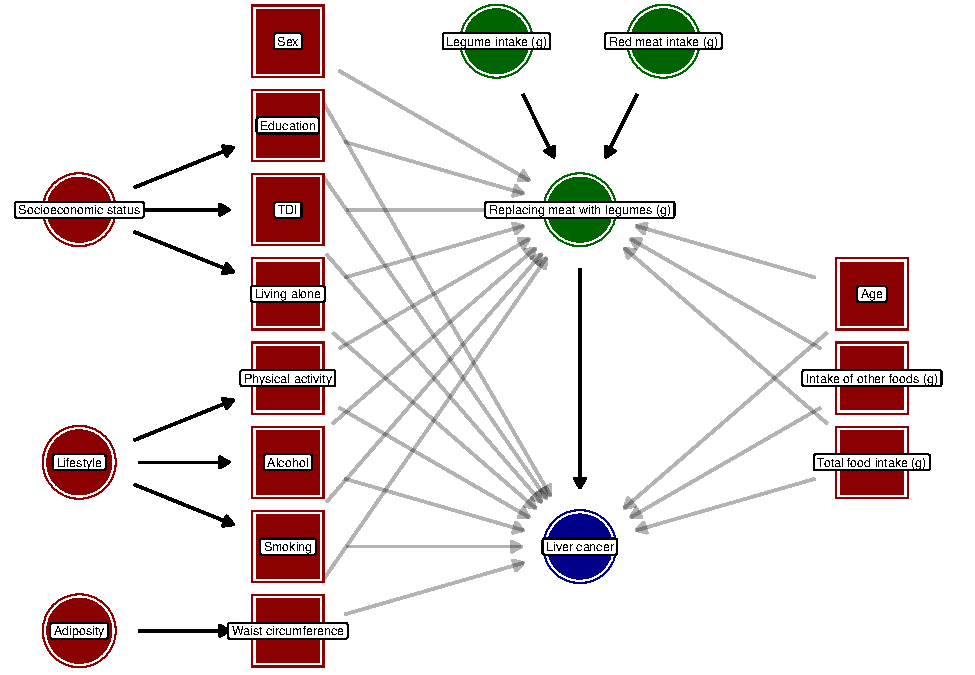
\includegraphics[width=1\linewidth,]{Springer-test_files/figure-latex/fig2-1} \caption{Directed acyclic graph (DAG) visualizing the hypothesised causal relationship between replacing red meat with legumes and liver cancer based on assumptions of biasing paths. Red nodes represent confounders. Square nodes represent the minimal sufficient adjustment set for estimating the effect of replacing red meat with legumes on liver cancer. Shadowed arrows represent biasing paths. DAG terminology demands visualisation of all hypothesized correlating relationships between variables, typically resulting in complex an hard-to-follow illustrations. To improve readability, inter-covariate arrows are hidden in the above DAG.}\label{fig:fig2}
\end{figure}

\newpage

\begingroup
\setlength\LTleft{0\linewidth}
\setlength\LTright{0\linewidth}\fontsize{9.8pt}{11.7pt}\selectfont
\begin{longtable}{@{\extracolsep{\fill}}>{\raggedright\arraybackslash}p{\dimexpr 0.2\linewidth-2\tabcolsep-1.5\arrayrulewidth}>{\raggedright\arraybackslash}p{\dimexpr 0.8\linewidth-2\tabcolsep-1.5\arrayrulewidth}}
\caption*{
{\large \textbf{Supplementary table 1. Summary of included foods for each food group.}}
} \\ 
\toprule
\textbf{Food group} & \textbf{Includes} \\ 
\midrule\addlinespace[2.5pt]
{\bfseries Legumes} & Soya-based desserts, Baked beans, pulses, Soya drinks (including calcium fortified),
  Tofu-based products, Hummus, Peas \\ 
{\bfseries Red meat} & Beef, Lamb, Other meat including offal, Pork \\ 
{\bfseries Processed meat} & Sausages, bacon (with and without fat), ham, liver pate \\ 
{\bfseries Animal-based foods} &   \\ 
Poultry & Fried poultry with batter/breadcrumbs, Poultry (with/without skin) \\ 
Fish & Fried fish with batter/breadcrumbs, Oily fish, including salmon, Prawns, lobster, crab, shellfish,
  Tinned tuna, white fish, other fish \\ 
Dairy & Spreadable/lower fat butter, dairy-based very low fat spread, Spreadable normal fat butter, dairy-based normal fat spread (including cholesterol lowering spread),
  Ice cream, milk puddings, milk-based desserts, cheesecake, Dairy-based smoothies, milk-based drinks, hot chocolate,
  Whole milk yogurt (plain), Cheese >17.5 g fat per 100 g, including hard cheese, soft cheese, spreadable, Blue, Feta, Mozzarella, Goats, other),
  Fat free and lower fat yogurt, plain or flavoured, Cheese <=17.5g fat per 100 g, including hard and spreadable lower fat cheese, Cottage,
  Semi-skimmed milk >1 g fat per 100 g (cow, other), Skimmed milk <1 g fat per 100 g (cow, cholesterol lowering, powdered),
  Whole milk >3.6 g fat per 100 g (cow, goat, sheep), Cream (cow's milk) \\ 
Eggs & Whole eggs and processed (omelette, scotch eggs, other) \\ 
Sauces & Mayonnaise, salad dressing, pesto, cheese sauce, white sauce, gravy, Yeast, chutney, olives, ketchup, brown sauce, tomato sauce \\ 
Mixed dishes & Pizza (including gluten free crust), Crisps, savoury biscuits, cheese snacks, other savoury biscuits,
  Soups, homemade, powdered and canned, Sushi \\ 
{\bfseries Healthy plant-based foods} &   \\ 
Whole grains & Mixed, brown or seeded bread, sliced, baguette, bap, roll, Wholemeal bread, sliced, baguette, bap, roll,
  Wholewheat biscuit cereal, Bran cereal, Porridge oats (including milk/dried fruit added),
  Oatcrunch breakfast cereal, Muesli (with or without dried fruit), Brown and wholemeal pasta and rice \\ 
Fruits & Apples and pears, Blackberries, strawberries, blueberries, raspberries, cherries, Grapefruit, orange, satsuma,
  Dried fruit, prunes, Bananas, mixed fruit, grapes, mango, melon, peach, pineapple, kiwi, other, Stewed fruit, plums \\ 
Nuts & Peanut-butter and chocolate-based spread, Unsalted peanuts and nuts, Salted peanuts and nuts \\ 
Plant oils & Olive oil, Olive oil based lower fat spread, plant-based lower fat margarine and soya-based lower fat spread (including cholesterol lowering spread),
  Olive oil based spread, plant-based soft or hard margarine and soya-based spread (including cholesterol lowering spread) \\ 
Beverages & Normal instant, filter, cappuccino, espresso coffee, Decaffeinated instant, filter, cappuccino, espresso coffee,
  Black, green and other tea, Decaffeinated black, herbal tea, rooibos, Plain water, sparkling water \\ 
Vegetables & Garlic, leek, onion, Broccoli, cabbage, kale, cauliflower, spinach, sprouts, Mixed side salad, lettuce, watercress,
  Beetroot, carrots, celery, parsnip, turnip, Fresh and tinned tomatoes,
  Mushrooms, mixed vegetables, avocado, broad beans, green beans, butternut squash, courgettes, peppers, other,
  Coleslaw, salad with added fat/mayonnaise, guacamole, sweetcorn \\ 
{\bfseries Unhealthy plant-based foods} &   \\ 
Refined cereals & Chocolate biscuits, plain biscuits, sweet biscuits and cookies, Naan, garlic bread, other bread (including gluten free),
  White bread, sliced, baguette, bap, roll, Oatcrunch breakfast cereal, Crisps, savoury biscuits, cheese snacks, other savoury biscuits,
  White pasta, rice, couscous, gluten free pasta \\ 
Potatoes & Potatoes, sweet potatoes, boiled or baked, Potatoes and chips, fried or roasted with fat, Potatoes, mashed \\ 
Fruit juice & Orange, grapefruit drink and 100\% fruit juice \\ 
Mixed dishes, vegetarian & Double and single crust pies, crumble pies, Yorkshire pudding, snackpot noodles,
  Indian samosa, pakora snacks, Quorn-based and vegetarian burgers and products \\ 
Sweets \& snacks & Table sugar, honey, jam and preserves,
  Chocolate bar (including white, milk and dark chocolate), chocolate-covered raisins, chocolate-covered sweets,
  Pancakes, croissant, Danish pastries, scones, fruitcakes, cakes, doughnuts, sponge puddings, other desserts, cereal bars, sweet snacks,
  Hard and soft sweets (including sugar free) \\ 
Sugar sweetened beverages & Rice and oat vegetable drinks, Low calorie fizzy drinks and squash, Fizzy sugary drinks, squash, fruit smoothies \\ 
{\bfseries Alcoholic beverages} & Beer and cider, Spirits and other alcoholic drinks, Fortified wine, Red and rose wine, White wine \\ 
\bottomrule
\end{longtable}
\endgroup

\newpage

\begingroup
\setlength\LTleft{0\linewidth}
\setlength\LTright{0\linewidth}\setlength{\LTpost}{0mm}
\begin{longtable}{@{\extracolsep{\fill}}lcc}
\caption*{
{\large \textbf{Supplementary table 2. Substitution of total meat, red meat and processed meat with legumes and hazard ratios and 95\% confidence intervals for hepatocellular carcinoma and intrahepatic cholangiocarcinoma.}}
} \\ 
\toprule
 & \textbf{Model 1}\textsuperscript{\textit{1}} & \textbf{Model 2}\textsuperscript{\textit{2}} \\ 
\cmidrule(lr){2-2} \cmidrule(lr){3-3}
\textbf{15 g/day of legumes replacing:} & \textbf{HR} \textbf{(95\% CI)} & \textbf{HR} \textbf{(95\% CI)} \\ 
\midrule\addlinespace[2.5pt]
\multicolumn{3}{l}{{\bfseries Hepatocellular carcinoma}} \\ 
\midrule\addlinespace[2.5pt]
Total red meat & 1.01 (0.93-1.10) & 1.06 (0.97-1.16) \\ 
Unprocessed red meat & 1.01 (0.92-1.11) & 1.05 (0.96-1.15) \\ 
Processed red meat & 1.01 (0.88-1.16) & 1.09 (0.95-1.26) \\ 
\midrule\addlinespace[2.5pt]
\multicolumn{3}{l}{{\bfseries Intrahepatic cholangiocarcinoma}} \\ 
\midrule\addlinespace[2.5pt]
Total red meat & 0.94 (0.87-1.02) & 0.97 (0.90-1.05) \\ 
Unprocessed red meat & 0.92 (0.85-1.00) & 0.95 (0.87-1.03) \\ 
Processed red meat & 1.02 (0.89-1.17) & 1.07 (0.93-1.22) \\ 
\bottomrule
\end{longtable}
\begin{minipage}{\linewidth}
\textsuperscript{\textit{1}}Adjusted for age (as underlying timescale), other food groups, and total food intake.\\
\textsuperscript{\textit{2}}Further adjusted for sex, educational level, Townsend deprivation index, living alone, physical activity, smoking, alcohol intake, and waist circumference.\\
\end{minipage}
\endgroup

\newpage

\begingroup
\setlength\LTleft{0\linewidth}
\setlength\LTright{0\linewidth}\setlength{\LTpost}{0mm}
\begin{longtable}{@{\extracolsep{\fill}}lccc}
\caption*{
{\large \textbf{Supplementary table 3. No intake of legumes vs. quartiles of daily legume intake and hazard ratios and 95\% confidence intervals for primary liver cancer.}}
} \\ 
\toprule
 &  & \textbf{Model 1}\textsuperscript{\textit{1}} & \textbf{Model 2}\textsuperscript{\textit{2}} \\ 
\cmidrule(lr){3-3} \cmidrule(lr){4-4}
\textbf{Characteristic} & \textbf{Mean daily legume intake} & \textbf{HR} \textbf{(95\% CI)} & \textbf{HR} \textbf{(95\% CI)} \\ 
\midrule\addlinespace[2.5pt]
Categories: &  &  &  \\ 
    No intake & 0.00 & — & — \\ 
    Q1 & 6.3 & 0.58 (0.35-0.96) & 0.59 (0.35-0.98) \\ 
    Q2 & 16 & 0.87 (0.56-1.33) & 0.89 (0.58-1.36) \\ 
    Q3 & 34 & 0.75 (0.47-1.19) & 0.75 (0.47-1.19) \\ 
    Q4 & 109 & 0.98 (0.64-1.51) & 1.06 (0.69-1.64) \\ 
\bottomrule
\end{longtable}
\begin{minipage}{\linewidth}
\textsuperscript{\textit{1}}Adjusted for age (as underlying timescale), other food groups, and total food intake.\\
\textsuperscript{\textit{2}}Further adjusted for sex, educational level, Townsend deprivation index, living alone, physical activity, smoking, alcohol intake, and waist circumference.\\
\end{minipage}
\endgroup

\newpage

\begin{landscape}

\begingroup
\setlength\LTleft{0\linewidth}
\setlength\LTright{0\linewidth}\fontsize{7.5pt}{9.0pt}\selectfont
\setlength{\LTpost}{0mm}
\begin{longtable}{@{\extracolsep{\fill}}>{\raggedright\arraybackslash}p{\dimexpr 0.1\linewidth-2\tabcolsep-1.5\arrayrulewidth}>{\centering\arraybackslash}p{\dimexpr 0.1\linewidth-2\tabcolsep-1.5\arrayrulewidth}>{\centering\arraybackslash}p{\dimexpr 0.1\linewidth-2\tabcolsep-1.5\arrayrulewidth}>{\centering\arraybackslash}p{\dimexpr 0.1\linewidth-2\tabcolsep-1.5\arrayrulewidth}>{\centering\arraybackslash}p{\dimexpr 0.1\linewidth-2\tabcolsep-1.5\arrayrulewidth}>{\centering\arraybackslash}p{\dimexpr 0.1\linewidth-2\tabcolsep-1.5\arrayrulewidth}>{\centering\arraybackslash}p{\dimexpr 0.1\linewidth-2\tabcolsep-1.5\arrayrulewidth}>{\centering\arraybackslash}p{\dimexpr 0.1\linewidth-2\tabcolsep-1.5\arrayrulewidth}}
\caption*{
{\large \textbf{Supplementary table 4. Sensitivity analyses}}
} \\ 
\toprule
 & \multicolumn{5}{c}{\textbf{Exclusion of participants with:}} &  &  \\ 
\cmidrule(lr){2-6}
 & \textbf{High alcohol intake}\textsuperscript{\textit{1}} & \textbf{Implausible food intake}\textsuperscript{\textit{2}} & \textbf{Liver disease before baseline}\textsuperscript{\textit{3}} & \textbf{Any cancer before baseline}\textsuperscript{\textit{4}} & \textbf{Fewer than 3 Oxford WebQs} & \textbf{Death register as source of liver cancer events} & \textbf{Exclusion of waist circumference from analysis} \\ 
\cmidrule(lr){2-2} \cmidrule(lr){3-3} \cmidrule(lr){4-4} \cmidrule(lr){5-5} \cmidrule(lr){6-6} \cmidrule(lr){7-7} \cmidrule(lr){8-8}
\textbf{15 g/day of legumes replacing:} & \textbf{HR} \textbf{(95\% CI)} & \textbf{HR} \textbf{(95\% CI)} & \textbf{HR} \textbf{(95\% CI)} & \textbf{HR} \textbf{(95\% CI)} & \textbf{HR} \textbf{(95\% CI)} & \textbf{HR} \textbf{(95\% CI)} & \textbf{HR} \textbf{(95\% CI)} \\ 
\midrule\addlinespace[2.5pt]
Total red meat & 1.00 (0.94-1.07) & 1.02 (0.96-1.08) & 0.99 (0.93-1.06) & 1.04 (0.97-1.11) & 1.04 (0.97-1.12) & 1.02 (0.97-1.09) & 1.00 (0.94-1.06) \\ 
Unprocessed red meat & 0.99 (0.92-1.06) & 1.00 (0.94-1.06) & 0.97 (0.91-1.04) & 1.01 (0.94-1.09) & 1.02 (0.94-1.11) & 1.01 (0.95-1.07) & 0.99 (0.92-1.05) \\ 
Processed red meat & 1.04 (0.93-1.17) & 1.09 (0.98-1.20) & 1.07 (0.96-1.20) & 1.15 (1.01-1.30) & 1.11 (0.97-1.27) & 1.07 (0.97-1.18) & 1.05 (0.95-1.16) \\ 
\bottomrule
\end{longtable}
\begin{minipage}{\linewidth}
\textsuperscript{\textit{1}}Exclusion of the upper 10th percentile of daily alcohol intake in grams for each sex.\\
\textsuperscript{\textit{2}}Exclusion of the upper and lower decile of daily energy intake for each sex.\\
\textsuperscript{\textit{3}}ICD10 codes: K70-79, B16-19, Z94.4, I82.0, I85, I86.4, E83.0-1 and E88. ICD9 codes: 571-574, 070, V427 and 2750-2751.\\
\textsuperscript{\textit{4}}ICD10 codes: C00-C97 and D00-D48. ICD9 codes: 140-239.\\
\end{minipage}
\endgroup

\end{landscape}

\newpage

\bibliography{bibliography.bib}


\end{document}
